\section{Photon counting}\label{sec:photon-counting}
We have already seen that the absorption of a single photon can generate a pulse in a photodetector. We can define the number of pulses per unit time, $N_r$, and the number of photons impinging on the detector per unit time, $N_p$. In general,
\[
N_r \leq N_p,
\]
because the detector quantum efficiency is smaller than or equal to one. In the linear regime, more precisely, one has
\[
N_r \simeq \eta\,N_p,
\]

where $\eta$ is the overall detection efficiency of the system.
\textbf{How do we count photons?}
\begin{itemize}
    \item The output signal consists of single voltage spikes superimposed on low- and high-frequency noise. These spikes correspond to individual detection events.
    \item The signal is fed into an amplifier, typically with a large gain, and low-frequency ripples are filtered out. This step improves the visibility of the real pulses with respect to the electronic background.
    \item The signal then enters a discriminator, which rejects pulses below a chosen threshold. In this way, pulses due to thermionic emission or other spurious effects can be removed.
    \item The accepted pulses are sent to a pulse shaper and then converted into a standard \textbf{TTL} (transistor-transistor logic) signal at the output.
    \item These TTL pulses are counted by an electronic counter and stored as digital information, namely as the number of pulses per unit time. If an analog output is needed, a digital-to-analog converter can be used.
\end{itemize}
For photon counting it is preferable to have:
\begin{enumerate}
    \item A short temporal width of the output pulse, so that individual events can be clearly separated from one another and from spurious pulses. Shorter pulses allow higher count rates, typically on the order of $10-20\,\mathrm{ns}$.
    \item A high quantum efficiency $\eta$ of the photocathode and a low anode dark current. This is essential to maximize the signal-to-noise ratio, since a high number of primary photoelectrons must be generated while thermally induced electrons must be minimized.
    \item An appropriate pulse-height distribution. The pulse heights corresponding to true signal events and to dark counts may overlap only partially, and in general the average amplitude of signal pulses is expected to be higher than that of dark pulses. 
    \begin{figure}[H]
        \centering
        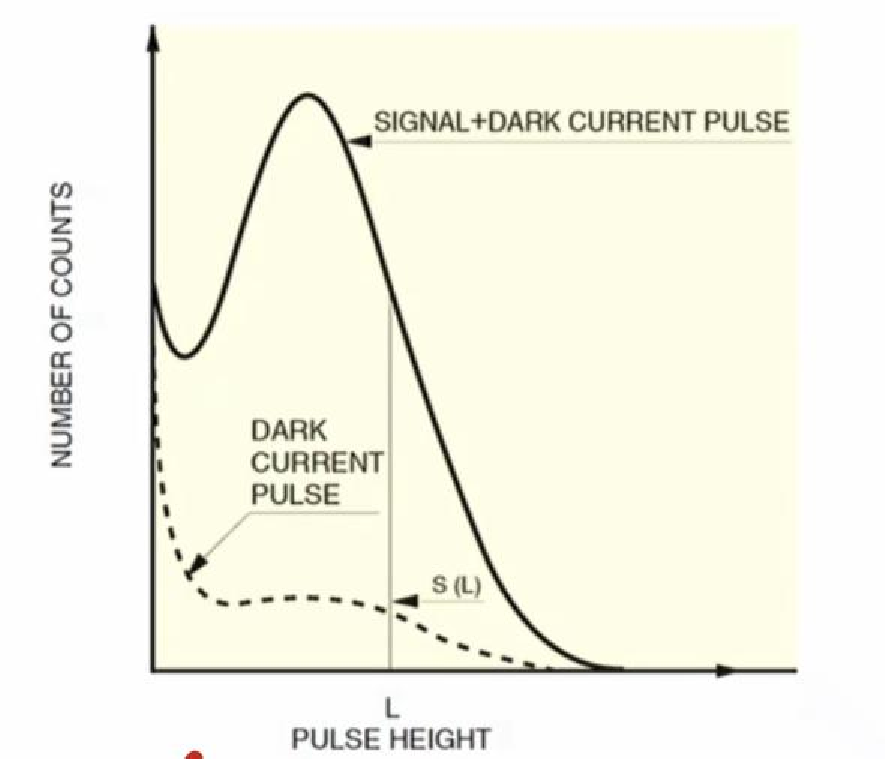
\includegraphics[width=0.4\linewidth]{images_in_pdf/9-/Grafico_48.pdf}
        \caption{Histogram of the occurrence of pulses with height $L$.}
    \end{figure}

    \item A careful choice of the photomultiplier voltage and of the discrimination threshold. If the count rate is measured as a function of the supply voltage, the signal typically increases faster than the noise at sufficiently high voltages. This happens because the discriminator suppresses a large fraction of the dark counts; only after the threshold voltage $V_0$ is reached does the signal-to-noise ratio saturate and approach a plateau.
    \begin{figure}[H]
        \centering
        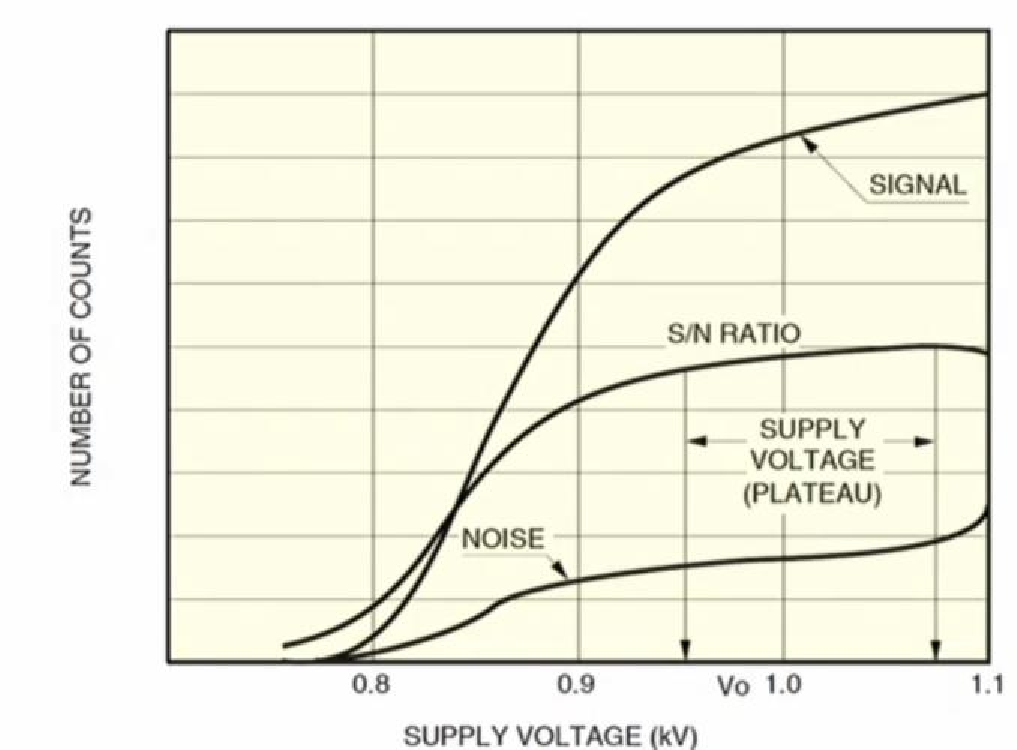
\includegraphics[width=0.4\linewidth]{images_in_pdf/9-/Grafico_49.pdf}
    \end{figure}

\end{enumerate}

\subsection{Time-correlated photon counting}
Time-correlated photon counting is a technique based on the statistics of light emission following excitation by a short light pulse. After excitation, the luminescence signal builds up and then decays in time. The detector records the arrival times of single photons, that is, the times at which individual pulses appear at the output. Each pulse corresponds to a single photoelectron emitted at the photocathode.

\textbf{How does it work?}
\begin{enumerate}
    \item We define $t=0$ as the time when the excitation pulse is emitted.
    \item The excitation pulse is repeated many times, so that the luminescence process is observed over a large number of identical cycles. The goal is to reconstruct the temporal decay of the emitted light by building a histogram of the photon arrival times within time intervals $\Delta t$.
    \begin{figure}[H]
        \centering
        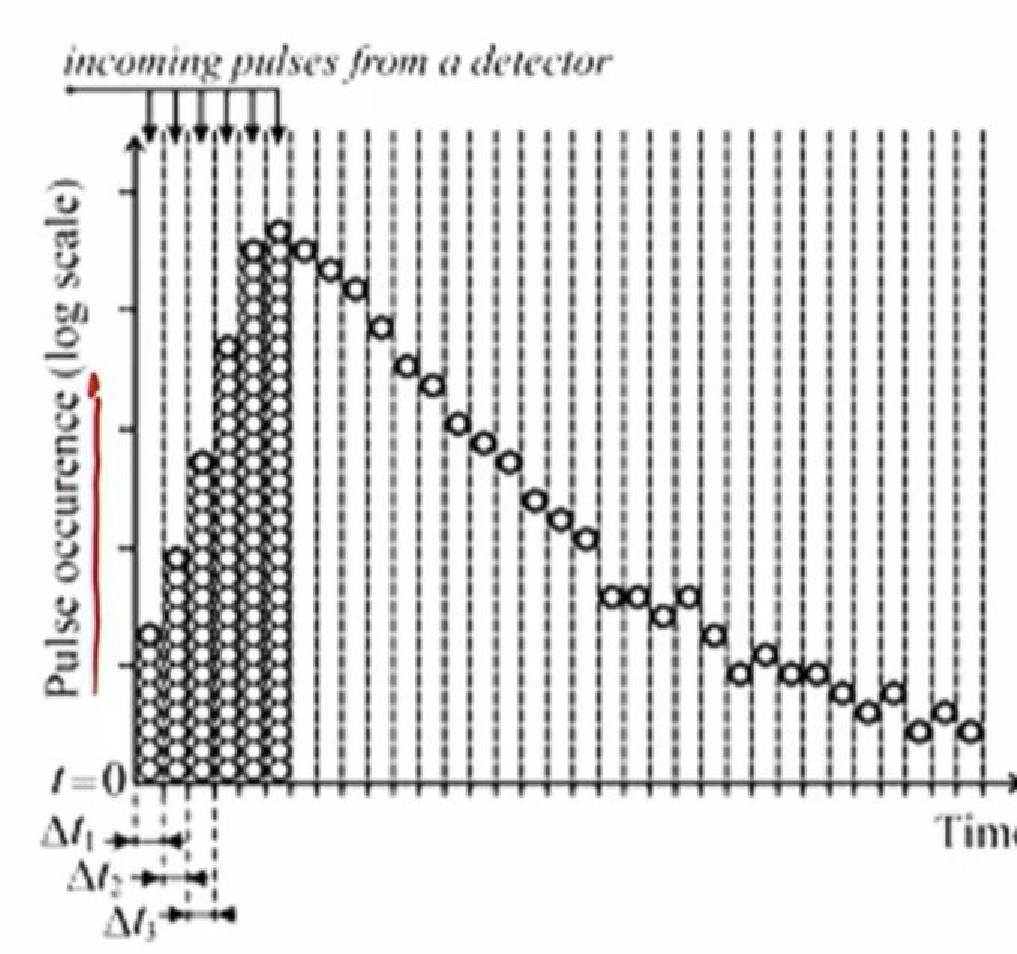
\includegraphics[width=0.4\linewidth]{images_in_pdf/9-/Grafico_50.pdf}
    \end{figure}

    The probability of detecting a photon at a given time is proportional to the number of fluorescence centers still in the excited state. As the experiment is repeated many times, the detection events are randomly distributed among the available time bins, and the accumulated histogram reproduces the decay law of the luminescence.
    
    To obtain reliable statistics, some conditions are required:
    \begin{itemize}
        \item The excitation intensity must be low enough to ensure that, on average, only one photon is detected per cycle, or at least that the probability of multiple detections per pulse remains small.
        \item A large number of events must be accumulated, so high repetition-rate lasers, typically in the kHz--MHz range, are used.
        \item A time-to-amplitude converter is employed. At $t=0$ the excitation pulse starts a linear voltage ramp; when the stop pulse arrives from the detector, the ramp is interrupted. The final voltage is proportional to the delay between the start and stop signals.
        This voltage is then sorted according to its amplitude and assigned to the corresponding channel of a multichannel analyzer. In this way, the number of events in each channel gives a histogram that is proportional to the photon arrival-time distribution, from which the characteristic lifetime can be extracted.
        \begin{figure}[H]
            \centering
            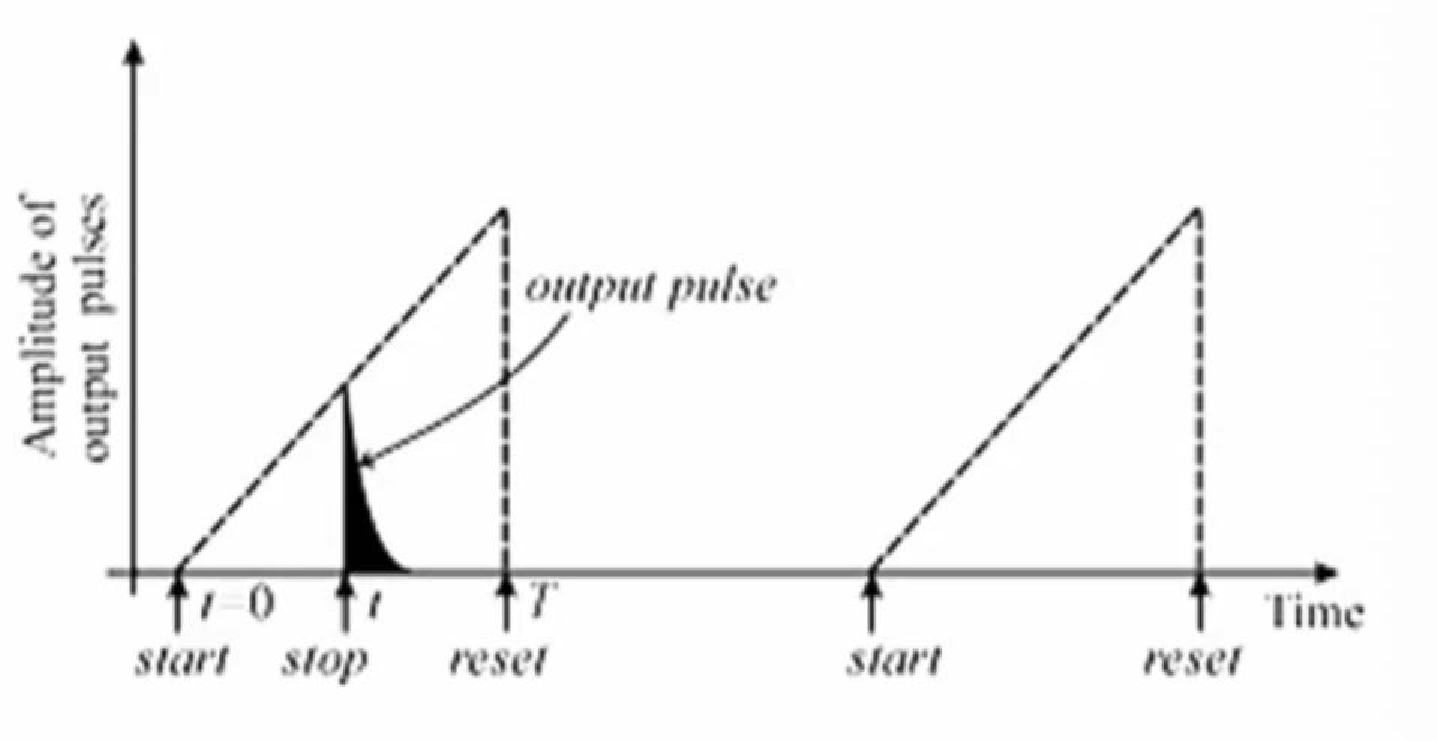
\includegraphics[width=0.4\linewidth]{images_in_pdf/9-/Grafico_51.pdf}
        \end{figure}

    \end{itemize}
\end{enumerate}